\documentclass[12pt]{article}
\usepackage{geometry}                % See geometry.pdf to learn the layout options. There are lots.
\geometry{letterpaper}                   % ... or a4paper or a5paper or ... 
%\geometry{landscape}                % Activate for for rotated page geometry
%\usepackage[parfill]{parskip}    % Activate to begin paragraphs with an empty line rather than an indent
\usepackage{graphicx}
\usepackage{amssymb}
\usepackage{subfig}
\usepackage{pstricks,pst-node,pst-tree}



\title{Analysis of loadings}
\author{Wesley Brooks}
\date{}                                           % Activate to display a given date or no date

\usepackage{Sweave}
\begin{document}
\setkeys{Gin}{width=0.9\textwidth}    %make figures a bit wider than the Sweave default.
\maketitle




First, we'll read the data files and divide the events into a few classes: one class for events that occured with snowmelt, one class for events that occured after the spring's last snowmelt but before mid-May (defined here as Julian date 135), and one class for events that occured after julian 135 and before the first snowmelt of the next winter. 

We also will look at dividing the data into just two groups: one that is snow-influenced and one that is not. "Not snow-influenced" just combines event classes two and three.\\











The next block of code produces a set of bar charts that show the relative contributions of the snow-driven events, post-snow-pre-vegetation events, and the post-vegetation events.\\











The next block prints a table of the proportion of total phosphorus loading due to each class of event at each site\\



% latex table generated in R 2.13.0 by xtable 1.5-6 package
% Fri Jun 17 18:25:28 2011
\begin{table}[h]
\begin{center}
\begin{tabular}{lccc}
  & snowmelt-driven & early post-snow & late post-snow \\ 
  \hline
eagle & 32.8\% & 22.9\% & 44.2\% \\ 
  joosvalley & 36.4\% & 16.9\% & 46.7\% \\ 
  otter & 45.9\% & 17.1\% & 37.0\% \\ 
  \end{tabular}
\caption{Proportion of total phosphorus loading contributed by each type of event}
\label{tab:ptot}
\end{center}
\end{table}
% latex table generated in R 2.13.0 by xtable 1.5-6 package
% Fri Jun 17 18:25:28 2011
\begin{table}[h]
\begin{center}
\begin{tabular}{lccc}
  & snowmelt-driven & early post-snow & late post-snow \\ 
  \hline
eagle & 27.0\% & 29.1\% & 43.9\% \\ 
  joosvalley & 26.9\% & 20.5\% & 52.6\% \\ 
  otter & 34.8\% & 21.0\% & 44.2\% \\ 
  \end{tabular}
\caption{Proportion of total suspended solids loading contributed by each type of event}
\label{tab:stot}
\end{center}
\end{table}








Produce plots of the proportion of the suspended solids and phosphorus (both total loading and stormflow loading) that is contributed by each class of event at each stream site:\\



\begin{figure}[h!]
    \begin{center}
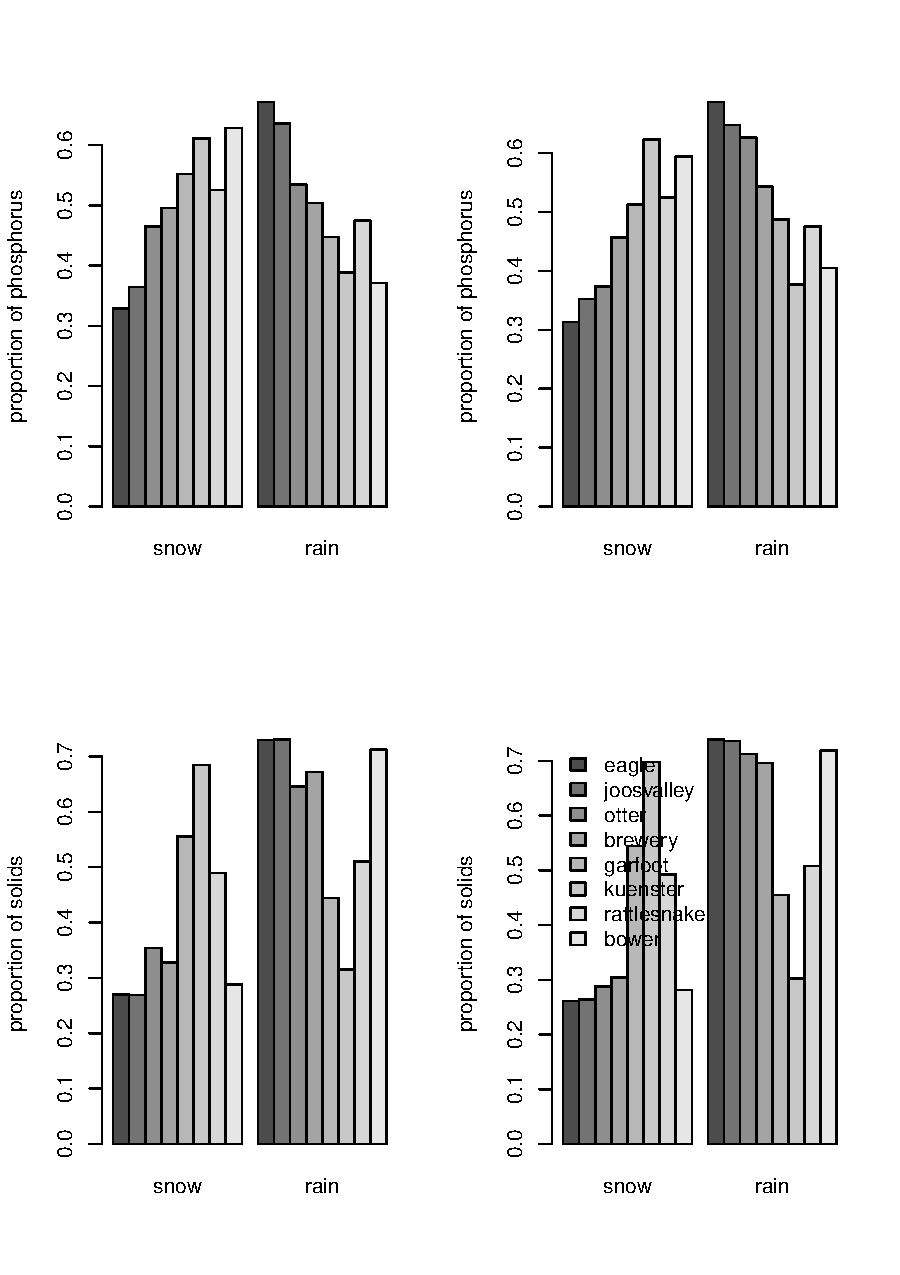
\includegraphics{loadings-fig2}
    \end{center}
    \vspace{-10mm}
    \caption{Cumulative storm loadings at the three creeks.\label{bars}}
\end{figure}



Now let's do the same between the snow and no-snow events:\\






Put the barchart into the document here:\\



\begin{figure}[h!]
    \begin{center}
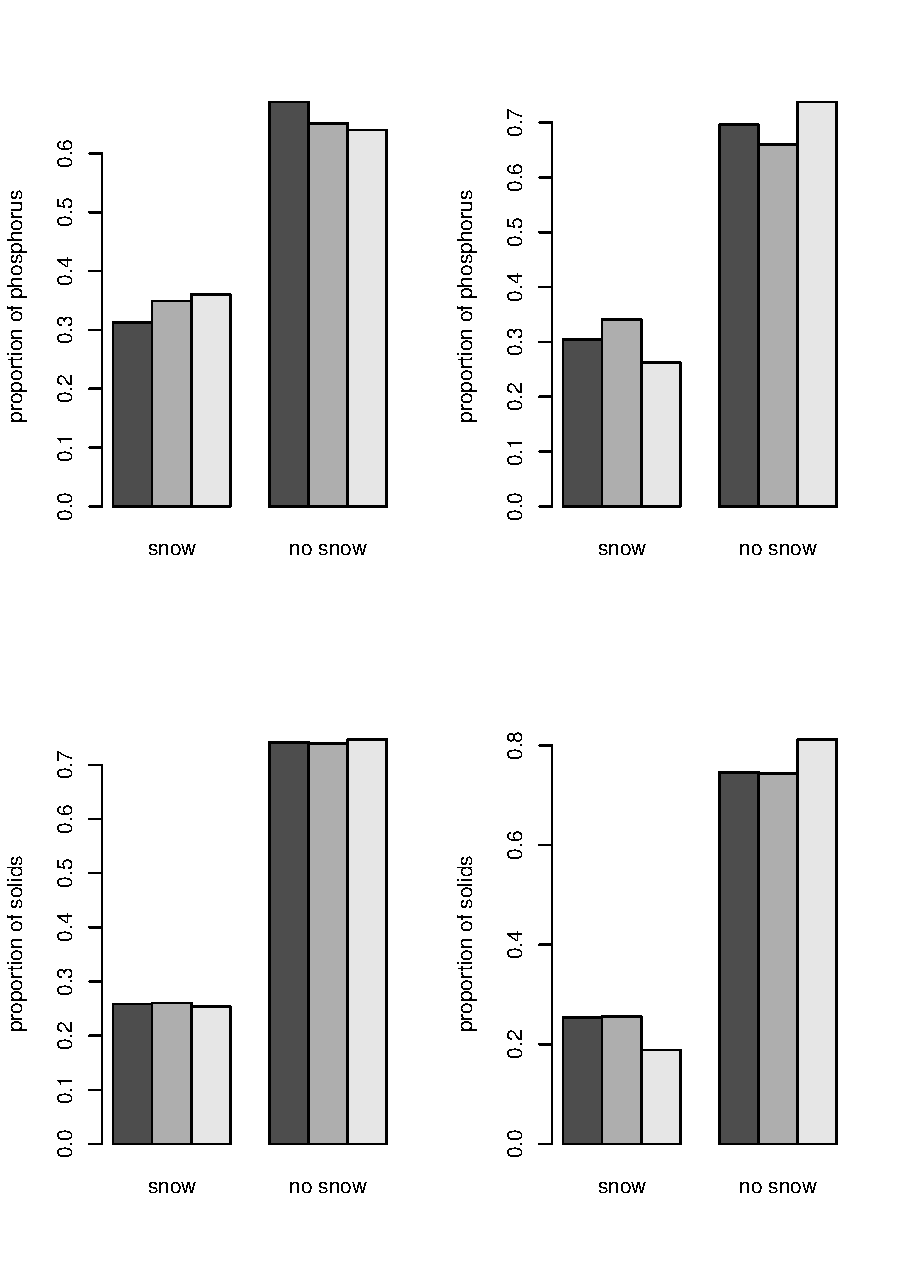
\includegraphics{loadings-fig3}
    \end{center}
    \vspace{-10mm}
    \caption{Cumulative storm loadings at the three creeks.\label{bars2}}
\end{figure}







%Boxplots of the contribution from individual storm events
\begin{figure}[h]
    \setkeys{Gin}{width=1\textwidth}    %make figures a bit wider than the Sweave default.
    \begin{center}
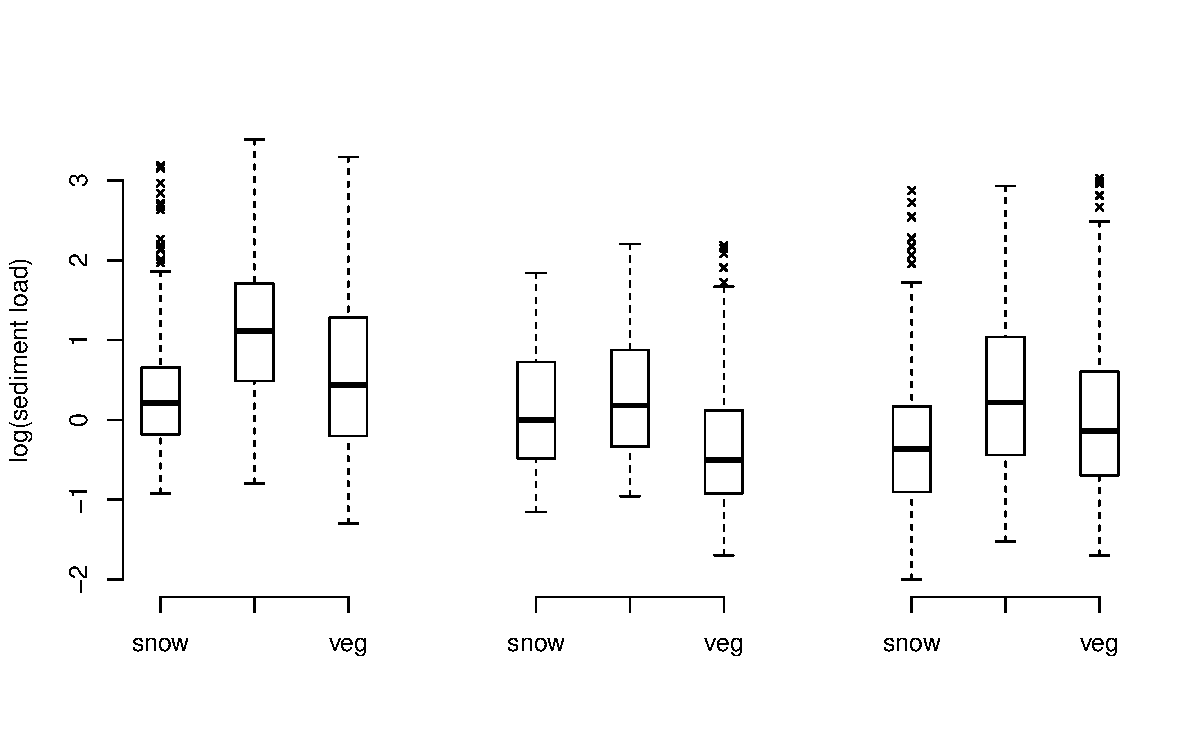
\includegraphics{loadings-boxplot_stot}

    \end{center}
\end{figure}







%Boxplots of the contribution from individual storm events
\begin{figure}[h]
    \setkeys{Gin}{width=1.1\textwidth}    %make figures a bit wider than the Sweave default.
    \begin{center}
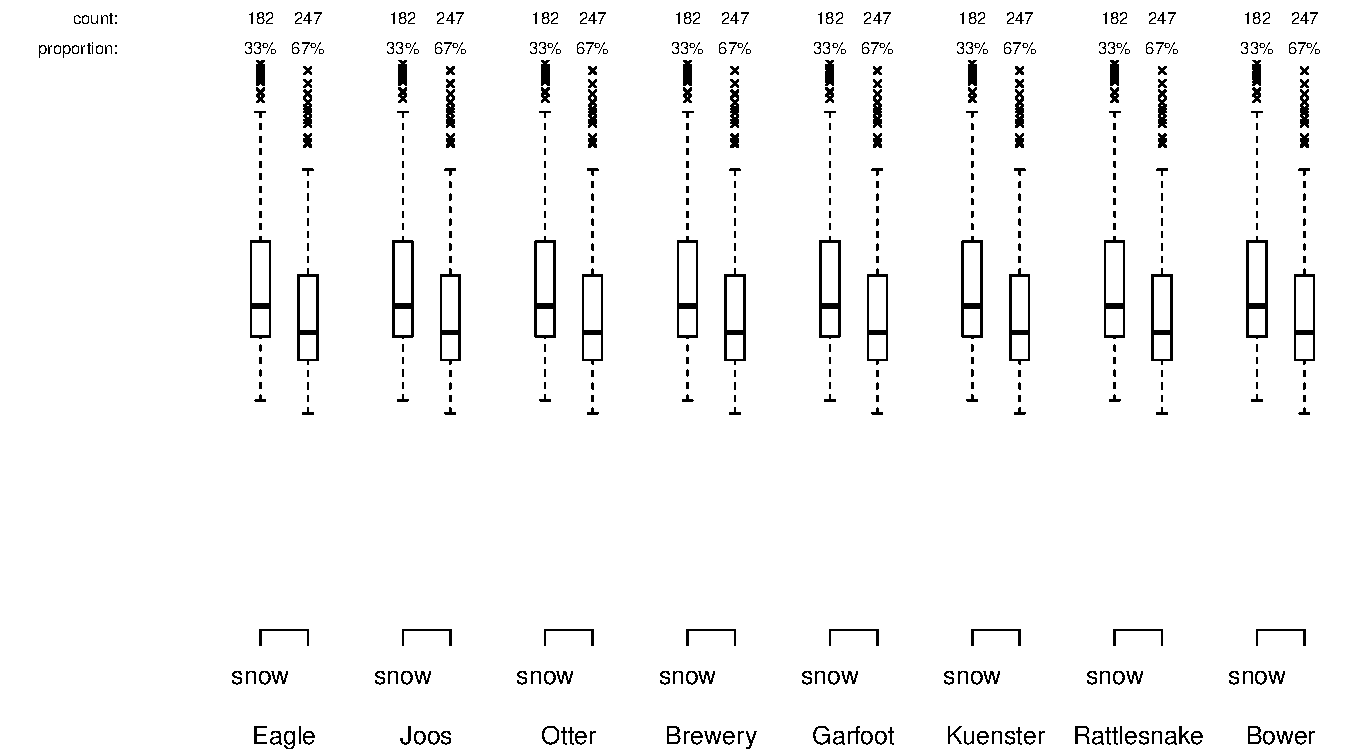
\includegraphics{loadings-boxplot_ptot}

    \end{center}
\end{figure}










\begin{figure}
    \begin{center}
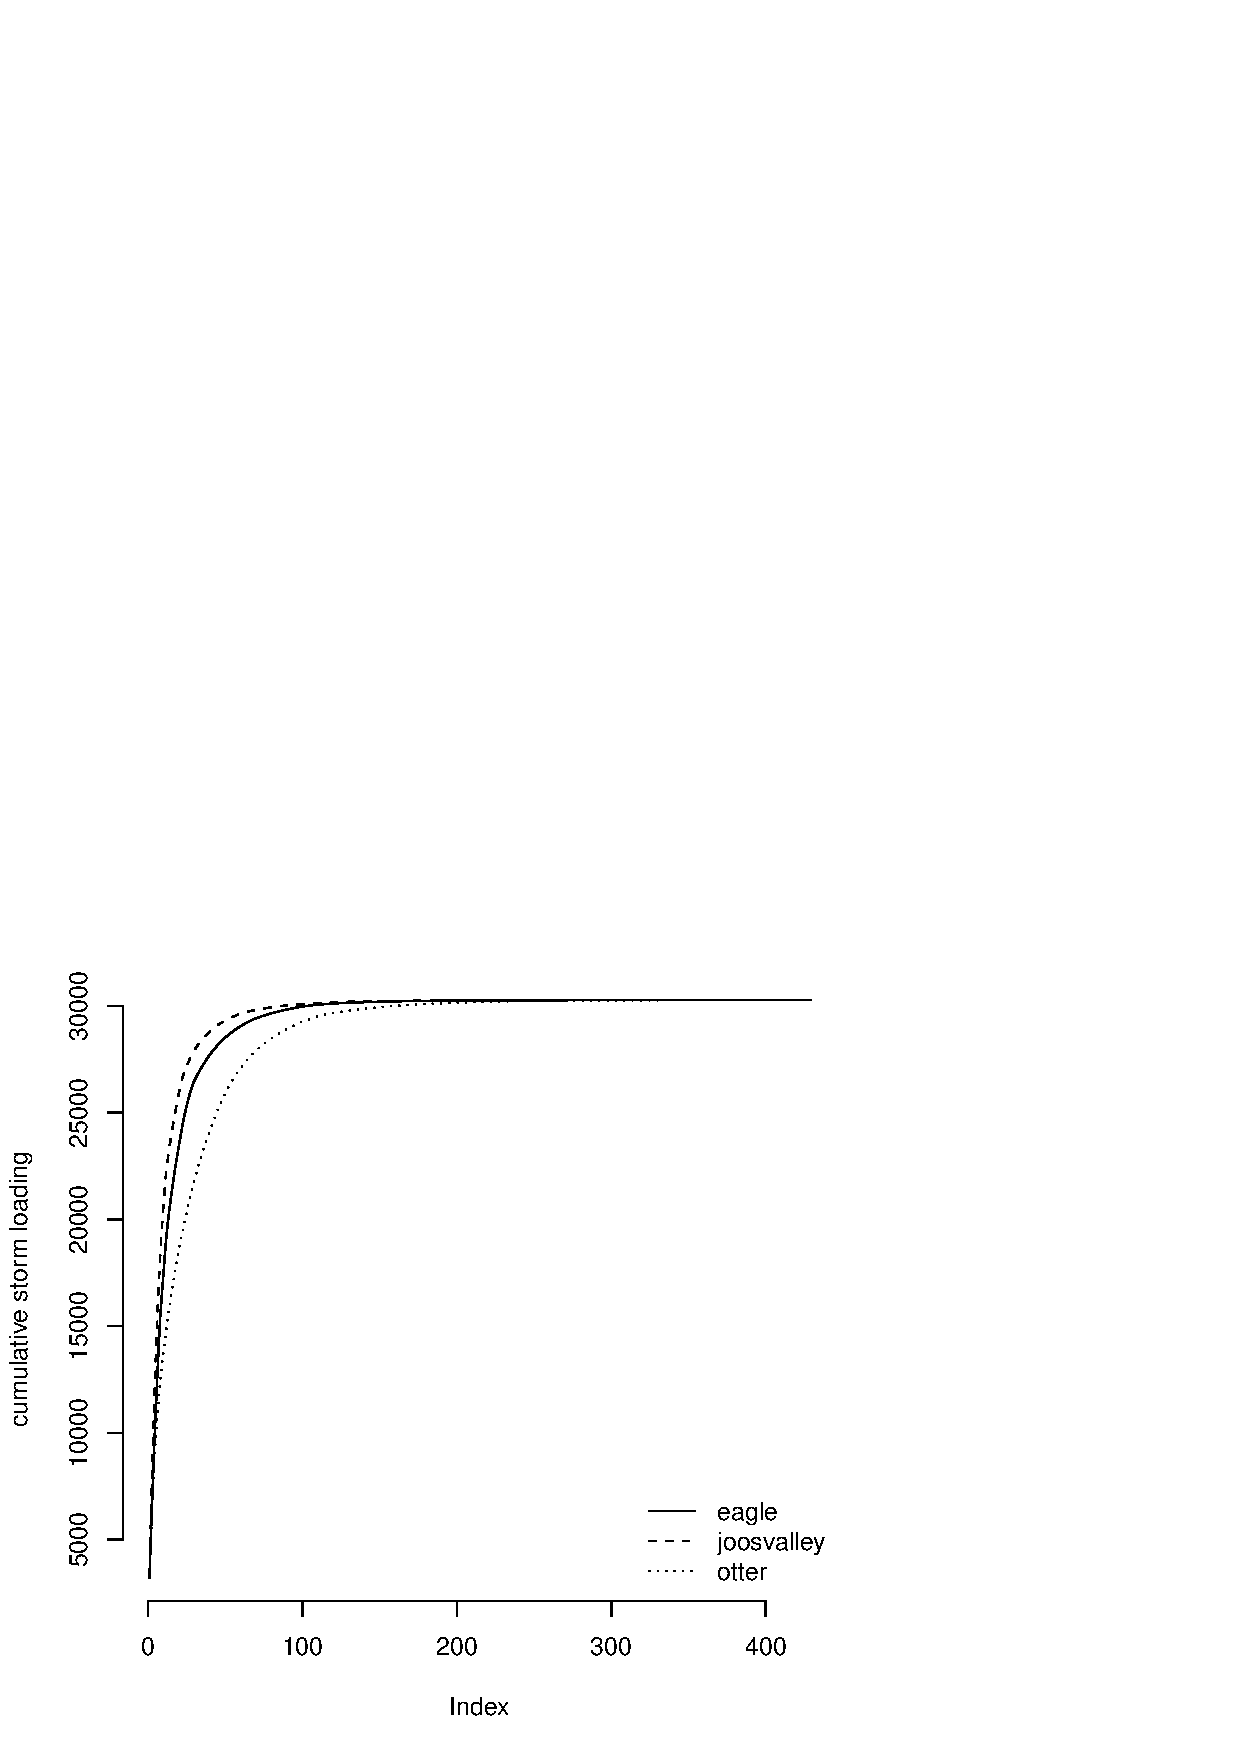
\includegraphics{loadings-figure1}
    \end{center}
    \caption{Cumulative storm loadings at the three creeks.\label{cdf}}
\end{figure}


\begin{figure}
    \begin{center}
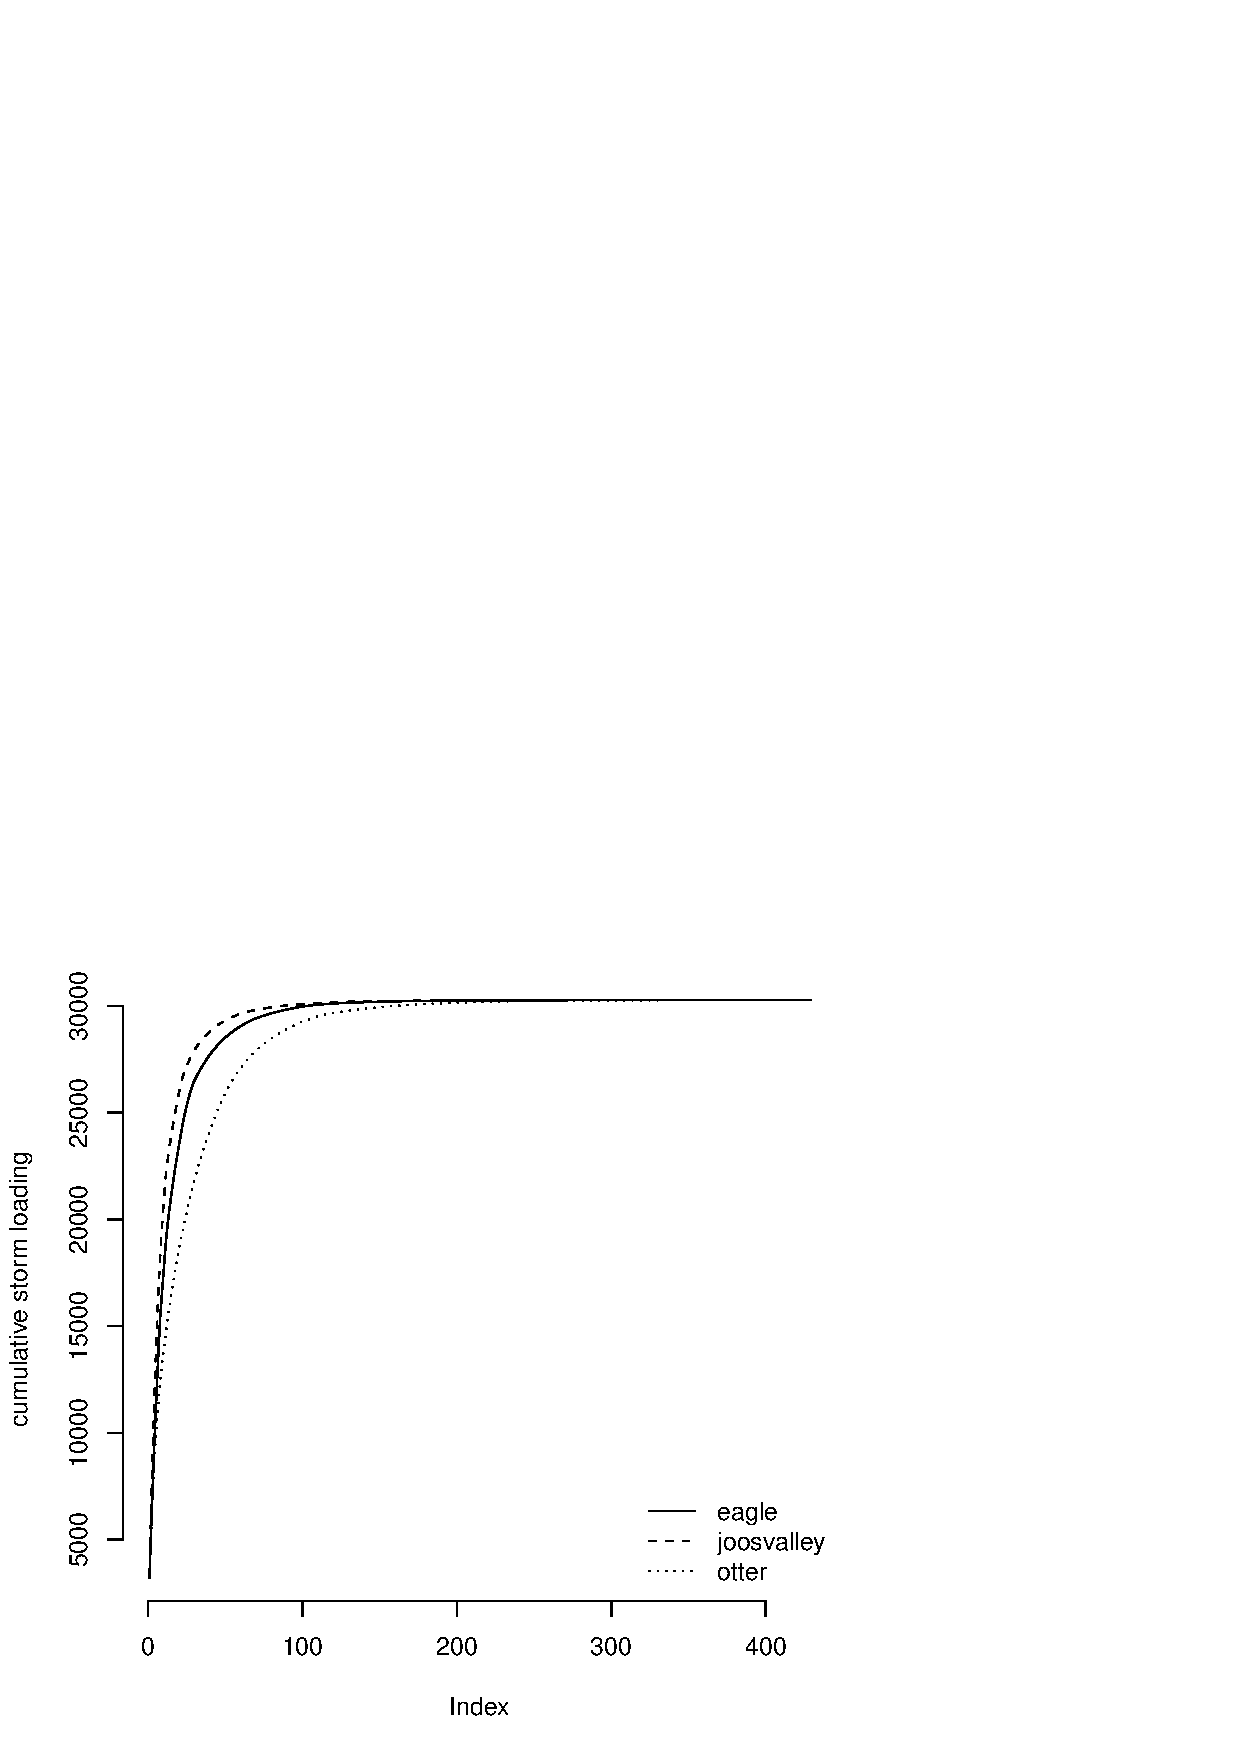
\includegraphics{loadings-figure1}
    \end{center}
    \caption{Proportion of the total sediment load contributed by rainfall events up to the size shown. Snowmelt-driven events are excluded.\label{cdf}}
\end{figure}

\begin{figure}
    \begin{center}
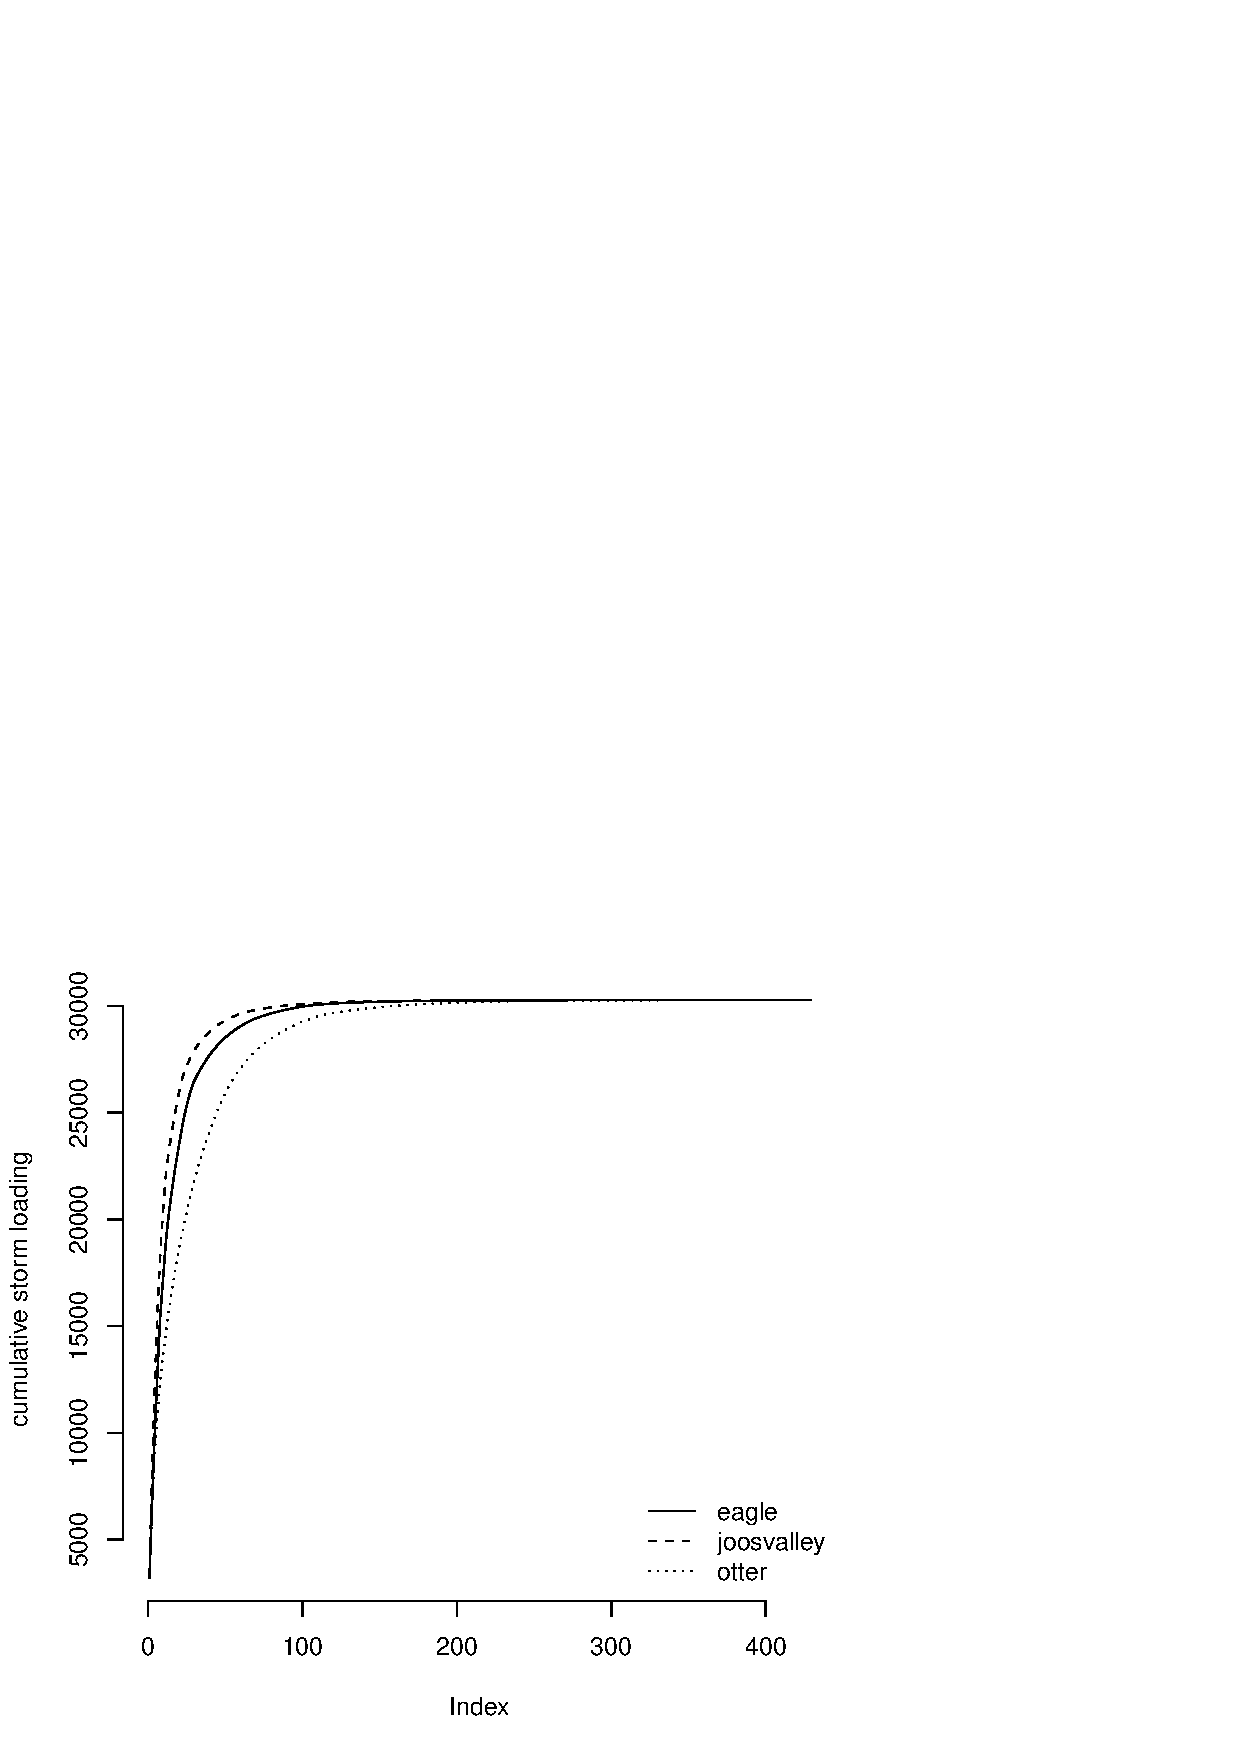
\includegraphics{loadings-figure1}
    \end{center}
    \caption{Proportion of the total phosphorus load contributed by rainfall events up to the size shown. Snowmelt-driven events are excluded.\label{cdf}}
\end{figure}



Figure out what proportion of total sediment loading is contributed by the top 10\% of storms:\\








The top 10\% of events contributed 89.1\% of the sediment loading at Eagle Creek, 73.1\% of the sediment loading at Otter Creek, and 93.4\% of the sediment loading at Joos Valley Creek.\\

Now we want to know how these major events are distributed within the event classes; that is, whether snowmelt tends to produce major loading events, or whether it is the post-snow events. Note that the \_tot column measures the total loading during an event. The snowmelt-driven events are different in kind than the rainfall-driven ones because they don't require continuous rain during the event. If the snowmelt-driven events are caused by warm weather, it seems reasonable that a single event might last for many days and cause more loading than a more-intense rainfall event that only lasts a day or two. To account for this, we will look both at total loading (\_tot) and average daily loading during an event (\_avg).\\


\begin{table}[h]
    \begin{center}
    \begin{tabular}{lr|lr|lr|l}
        & \multicolumn{2}{c}{Snowmelt    }\ & \multicolumn{2}{c}{Early post-snow}\ & \multicolumn{2}{c}{Late post-snow} \\
        Creek & All & Major & All & Major & All & Major \\
        \hline 
        Eagle & 42\% & 30\% & 13\% & 19\% & 45\% & 51\% \\
        Otter & 39\% & 42\% & 12\% & 19\% & 49\% & 40\% \\
        Joos & 46\% & 31\% & 11\% & 17\% & 43\% & 52\% \\
        
    \end{tabular}
    \end{center}
\end{table}



The table shows that the major loading events that produce the majority of the loading can be occur during each of the three annual periods. However, the events caused by snowmelt produced a smaller proportion of major events than their proportion of all events, and their relative contribution to the total sediment load was smaller than their proportion of loading events. Taken together, these insights tell us that, while snowmelt can cause a major loading event, a snowmelt-driven event is less likely to be a major contributor to sediment load than is a rainfall-driven event.\\

We can also see that the 43\% of the events were driven by snowmelt; these events contributed only 27\% of the total sediment load but 36\% of the total phosphorus load.

Meanwhile, the 12\% of events that were caused by early-season rainfall produced 27\% of the total sediment load and 20\% of the total phosphorus load.

Meanwhile, the 46\% of events that were caused by late-season rainfall produced 46\% of the total sediment load and 44\% of the total phosphorus load.


Overall, 34\% of the largest events at each site were produced by snowmelt; 18\% were produced by early-season rainfall, and 48\% were produced by late-season rainfall.



 %\begin{landscape}
 \begin{center}
\psset{linecolor=black,tnsep=2pt,tnheight=0cm,treesep=.3cm,levelsep=40pt,radius=10pt}
%     \def\psedge#1#2{\ncangle{#2}{#1}}
%     \pstree[treemode=R]
    \Tcircle[fillcolor=yellow,fillstyle=solid]{ 1 }~{\textit{48.34}}
 \end{center}
GUIDE piecewise constant least-squares regression tree model.
At each intermediate node, a case goes to the left branch 
  if and only if the condition is satisfied.
Number in italics beneath leaf node is sample mean of stottot.
 %\end{landscape} %\begin{landscape}
 \begin{center}
\psset{linecolor=black,tnsep=2pt,tnheight=0cm,treesep=.3cm,levelsep=40pt,radius=10pt}
%     \def\psedge#1#2{\ncangle{#2}{#1}}
%     \pstree[treemode=R]
    \Tcircle[fillcolor=yellow,fillstyle=solid]{ 1 }~{\textit{175.48}}
 \end{center}
GUIDE piecewise constant least-squares regression tree model.
At each intermediate node, a case goes to the left branch 
  if and only if the condition is satisfied.
Number in italics beneath leaf node is sample mean of stottot.
 %\end{landscape} %\begin{landscape}
 \begin{center}
\psset{linecolor=black,tnsep=2pt,tnheight=0cm,treesep=.3cm,levelsep=40pt,radius=10pt}
%     \def\psedge#1#2{\ncangle{#2}{#1}}
%     \pstree[treemode=R]
  \pstree{\Tcircle{ 1 }~[tnpos=l]{\shortstack[r]{theisen\\$\leq$ 2.20}}}{
  \pstree{\Tcircle{ 2 }~[tnpos=l]{\shortstack[r]{totalwater\\$\leq$ 1.98}}}{
    \Tcircle[fillcolor=yellow,fillstyle=solid]{ 4 }~{\textit{18.05}}
    \Tcircle[fillcolor=yellow,fillstyle=solid]{ 5 }~{\textit{272.43}}
   }
  \pstree{\Tcircle{ 3 }~[tnpos=l]{\shortstack[r]{tmean\\$\leq$ 68.50}}}{
    \Tcircle[fillcolor=yellow,fillstyle=solid]{ 6 }~{\textit{482.94}}
    \Tcircle[fillcolor=yellow,fillstyle=solid]{ 7 }~{\textit{685.43}}
 }
 }
 \end{center}
GUIDE piecewise constant least-squares regression tree model.
At each intermediate node, a case goes to the left branch 
  if and only if the condition is satisfied.
Number in italics beneath leaf node is sample mean of stottot.
 %\end{landscape}


\end{document}
